\section{Case Study}
In this section, we demonstrate that, with the metadata automatically normalized and generated using the techniques in previous section, we are able to implement a few applications that are generalizable from one building to another building without modification.

\subsection{Experimental Setup}
We implement \# applications and perform the analysis on three buildings from two campuses, and each building is installed with a different management system. Building A was built in mid-1990s using the system from Barrington ~\cite{}. Building B was recently built in 2005 using the Siements BACnet system~\cite{}. Building C is the newest building among the three using Trane's system~\cite{}, which was put into use from 2011. We collected all the available data readings from each building, covering temperature, humidity, co2 concentration, light intensity, air damper and valve postions, air volume, setpoints for various streams. The data used from each building was one-week data in June 2009, January 2012 and June 2013 respectively.

\begin{figure*}[h]
\centering
	\begin{subfigure}{0.33\textwidth}
                \centering
		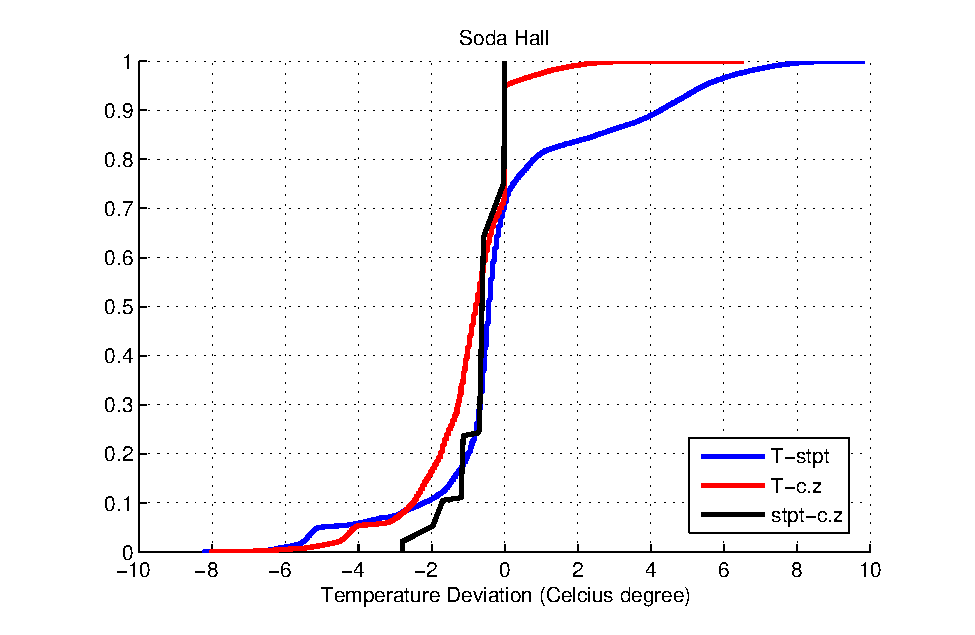
\includegraphics[width=\textwidth]{./figs/Soda_new.eps}
                \caption{Building A}
	\end{subfigure}
	\begin{subfigure}{0.33\textwidth}
                \centering
		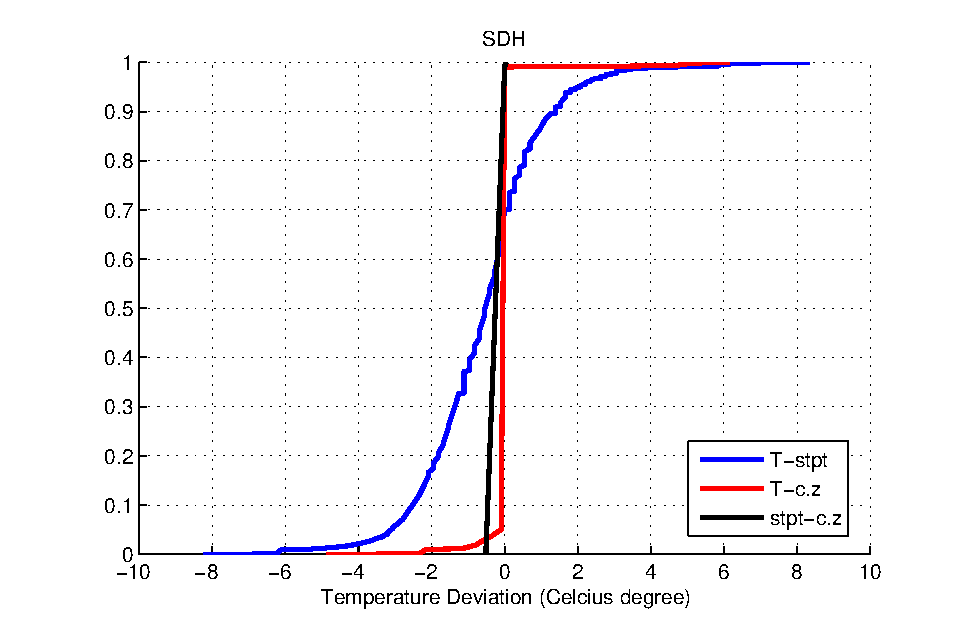
\includegraphics[width=\textwidth]{./figs/SDH_new.eps}
                \caption{Building B}
	\end{subfigure}
	\begin{subfigure}{0.33\textwidth}
                \centering
		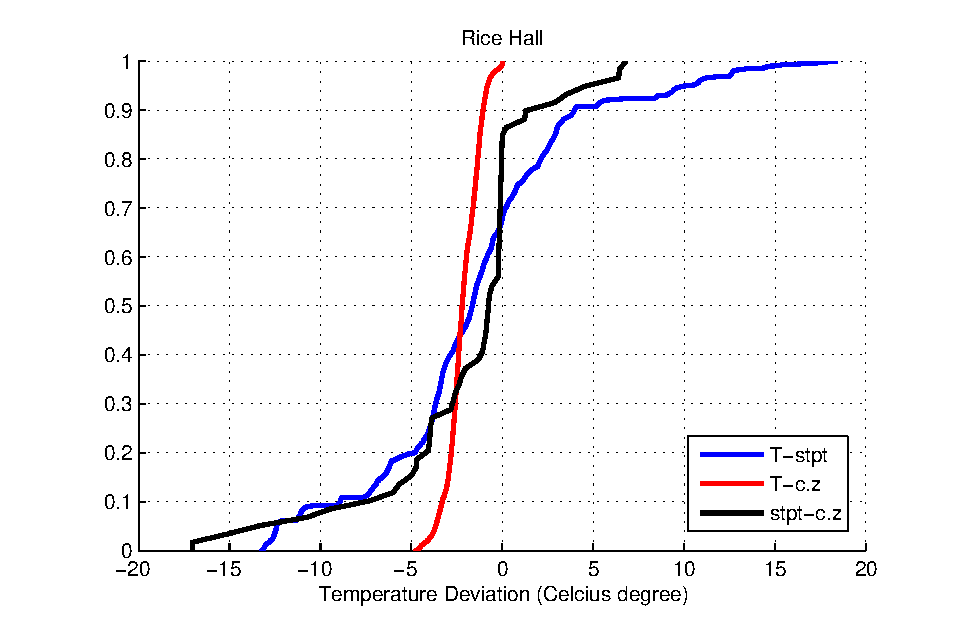
\includegraphics[width=\textwidth]{./figs/Rice_new.eps}
                \caption{Building C}
	\end{subfigure}
\caption{For each building, we present the distribution of temperature deviation between: a) room temperature and the corresponding setpoint (in blue), b) room temperature and the comfort range suggested by ASHRAE (in red), c) room temperature setpoint and the ASHARE comfort suggestion (in black).}
\label{fig:cdf_temp}
\end{figure*}


\subsection{Uncomfortable Rooms}
It's not unusual to have rooms in a building stay below or above the setpoint thus making the occupants feel uncomfortable as well as incurring energy waste. The temperature deviation could be caused by unproper setpoints or dysfunciton of the HVAC systems, and being able to identify these uncomfortable zones or rooms in the buildings is vital to occupant comfort. With the metadata normalized using our techniques, we are able to analyse the temperature parameters in different buildings without any modification to our applications. Specifically, we examine three different types of temperature deviations in a building: a) how much the temperature deviates from the setpoint; b) how much the temperature deviates from the comfort range suggested by ASHRAE; c) how much the temperature setpoint deviates from the ASHRAE comfort suggestion. We only consider the working hours from 9am to 5pm on weekdays for analysis and for each buidling, we accumulate the three different deviations for all the rooms and generate the CDF respectively as demonstrated in Figure~\ref{fig:cdf_temp}. We see that each buidling are uncomfortable to some degree and we are particularly interested in the periods when a room deviates from the setpoint more than 3 Celsius degree. Therefore, for each building, we zoom in to the interested portion and rank the rooms by their percentage of time that falls into the interested area, i.e., how much time the room temperature deviates from the setpoint more than 3 Celsius degree, and the results are summarized in Table~\ref (We only list the first ten rooms in each building).

\begin{table}[h!]
%\footnotesize
 \begin{center}
	\begin{tabular}{|c|c|c|c|c|c|}
	\multicolumn{2}{c}{$Bldg A$}
	 & \multicolumn{2}{c}{$Bldg B$}
	  & \multicolumn{2}{c}{$Bldg C$} \\
	\cline{1-6} 
	 330B & 1 & S3-6 & 1 & 501 & 1\\
	\cline{1-6}
	 340 & 1 & S2-1 & 1 & 502 & 1\\
	\cline{1-6}
	420A & 1 & S1-2 & 0.93 & 504 & 1\\
	\cline{1-6}
	420 & 1 & S7-16 & 0.67 & 557 & 1\\
	\cline{1-6}
	698 & 1 & S3-13 & 0.62 & 511A & 1\\
	\cline{1-6}
	442 & 0.996 & S4-15 & 0.62 & 532 & 1\\
	\cline{1-6}
	398 & 0.981 & S5-5 & 0.57 & 224 & 1\\
	\cline{1-6}
	336 & 0.96 & S4-1 & 0.54 & 506 & 1\\
	\cline{1-6}
	183 & 0.92 & S5-16 & 0.48 & 507 & 1\\
	\cline{1-6}
	498 & 0.91 & S5-7 & 0.47 & 511B & 1\\
	\cline{1-6}

	\end{tabular}
 \end{center}
 \caption{We rank the rooms in each building by the percentage of time when the temperature deviates from the setpoint more than 3 Celsius degree. The ranking helps identify the rooms that are likely to be rogue ones, i.e., which are under constant heating and cooling.}
 \label{tab:cluster}
\end{table}